\documentclass[12pt]{article}
\usepackage{mathptmx}
\usepackage[margin=1in]{geometry}
\linespread{2}

\usepackage{float}
\restylefloat{figure}
\usepackage{graphicx}
\usepackage{wrapfig}
\usepackage[font={scriptsize}]{caption}

\usepackage[backend=bibtex,style=mla]{biblatex}
\bibliography{citations.bib}

\author{5038-47626}
\title{Machine Learning and Sentiment Analysis\\Using Public Data}

\begin{document}
    \begin{titlepage}
        \pagenumbering{gobble}
        \maketitle
    \end{titlepage}
    \pagenumbering{arabic}
    \tableofcontents

        \section{Abstract}
        Machine Learning refers to building computer systems that are able to perform tasks normally performed by human brain and require human intelligence.  There are many applications of this emerging technology, including Sentiment Analysis. Sentiment Analysis refers to identifying emotion as expressed in a line of text. In this report, I have used Neural Network to model a human brain.  Much like a human brain, a neural network consists of a mesh of mathematical neurons interconnected with each other in an organized fashion so as to facilitate processing of information.  A mathematical neuron consists of one or more inputs and one output.  The inputs are multiplied by their respective weights and then added together to obtain a sum which is then compared against a threshold.  If a threshold is met, the neuron fires an output signal, else it suppresses it.  In this report, I have used a neural network to process a line of text and identify the emotion hidden in it.  Much like a human brain, such a neural network needs to be trained, which requires a huge amount of data and associated output emotions.  Since Twitter is full of sentimental text with hashtags identifying the contextual emotion expressed in the text, it makes it a perfect candidate for the training of my network.  Hence I gather the data from Twitter, train the network and then use a front end that I developed to demonstrate the idea.
        
    \section{Research Question}
    How to apply machine learning to sentiment analysis in order to estimate the emotion expressed within a text?

    \section{Introduction}
    Machine learning is a fast growing technology allowing for the processing of vast quantities of information quickly. Previous approaches to data processing required certain conditions that must be met to process the data, and these conditions had to be expressed in terms of absolutes. These approaches have limitations when it comes to processing data. For example, by reading a sentence, the brain can figure out what emotion has been expressed in the sentence. This refers to a topic in artificial intelligence called sentiment analysis. It is impossible to perform sentiment analysis using the traditional approaches, because emotions such as humor cannot be expressed absolutely. Machine Learning models a brain\autocite{MLVision} in order to process data (text in the case of sentiment analysis) and draw a conclusion (the sentiment expressed in the text)\autocite{GoldenAgeArchitecture}. There are many uses for sentiment analysis. Facebook, for example, uses it to decide what order to show your feed in. If it finds that you show positive sentiment towards a certain product or idea, it is weighted higher on your feed and vice versa. Google uses this to know what ads to serve you when on sites that use their ad service.

    \section{Neural Networks}
    \subsection{The Model}
    Machine learning is a technique for data processing that models a brain. This means anything a human can understand, a machine can too. This model is called a neural network, since it models neurons in the human brain. Fig.~\ref{fig:Neuron} shows the model of a neuron. 

    \begin{figure}
        \begin{center}
            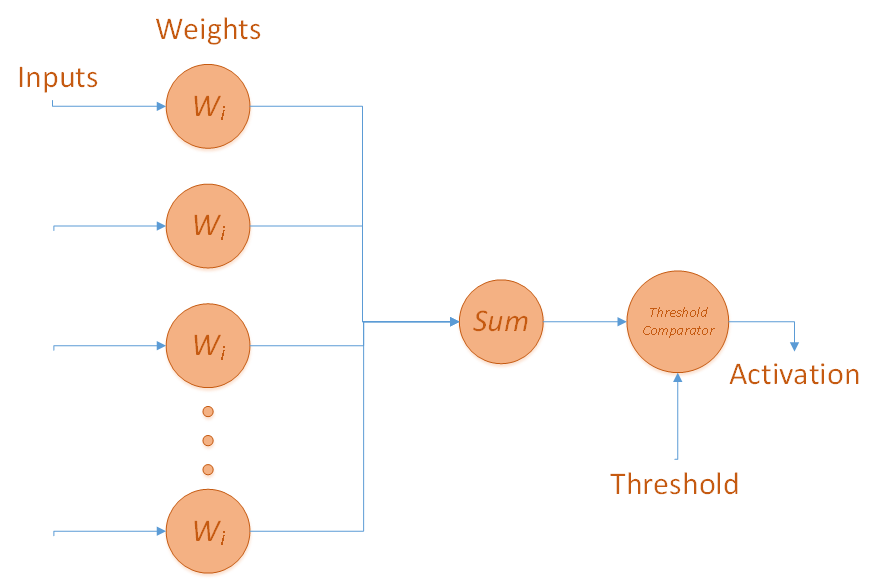
\includegraphics[width=5in]{Neuron.png}
        \end{center}
        \caption{Mathematical model of a neuron.}
        \label{fig:Neuron}
    \end{figure}

    A mathematical neuron, just like a real one in a brain, takes inputs from multiple neighboring neurons, multiplies them with corresponding weights, and then adds up the results as shown in the figure. The sum is then compared against a threshold. If the threshold is met, the neuron generates an output signal. If not, then it simply suppresses the signal. Whatever the output is, it is fed into other neurons as their input and they go through the same process. This interconnect of neurons is called a Neural Network and is shown in Fig.~\ref{fig:NN}.

    
    \begin{figure}
        \begin{center}
            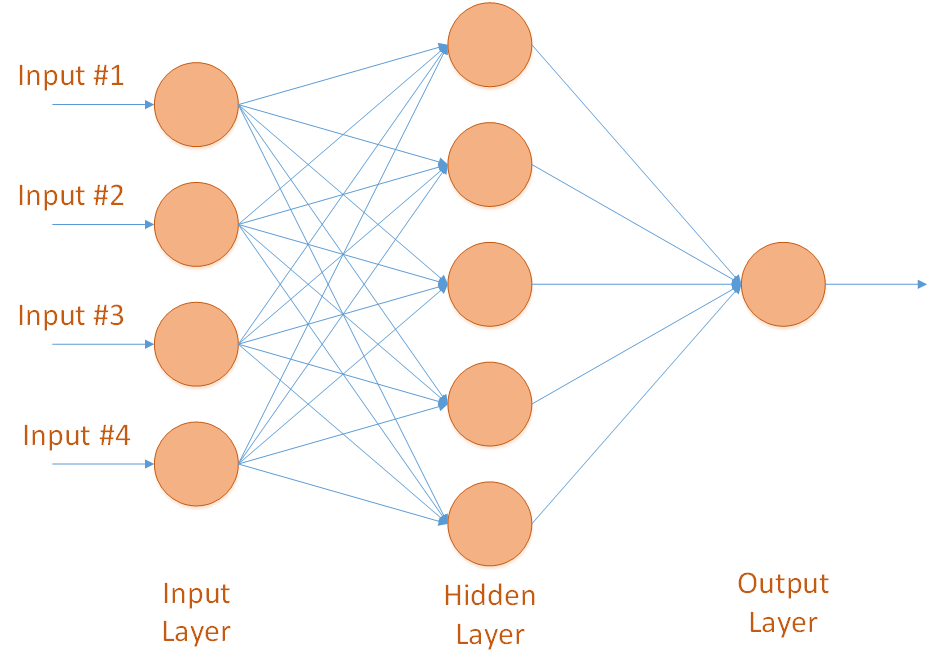
\includegraphics[width=5in]{Neural_Network.png}
        \end{center}
        \caption{A model of a neural network.}
        \label{fig:NN}
    \end{figure}
    
    \subsection{Training}
    Much like a human brain, a neural network requires training which is done by modifying the weights and thresholds of each neuron until the network has desirable results. This requires large quantities of data. Ways of getting this include using user inputted data on a service, harvesting data from user posts, and captchas which ask you to click on pictures that include certain items. This data also requires an answer key. For example, a neural network to tell if a post on facebook is happy or sad should be trained with data that includes sample posts and associated emotion for whether it is happy or sad. These sets of data known as datasets can consist of millions of entries.

    Each one of the entries within a dataset is fed through the network with random values for the weights and thresholds. These are then modified and then the entries are fed through the network again. If this modified network has more accurate results than the previous one, then the previous network is discarded and this new one is used. Otherwise, the previous one is used. This process repeats. This brute force method of training requires large amounts of compute power and time in order to have a well trained and accurate network.

    \section{Sentiment Analysis using Neural Networks}
    \subsection{Sentiment Analysis}
    Use cases for machine learning are hard to find. Since machine learning is not 100\% accurate, just like humans, if there is another way to solve the problem it is most likely a better method\autocite{pitfallsML}. So using machine learning to solve basic arithmetic is not a good use case. An example of a good use case, however is sentiment analysis.

    \begin{figure}
        \begin{center}
            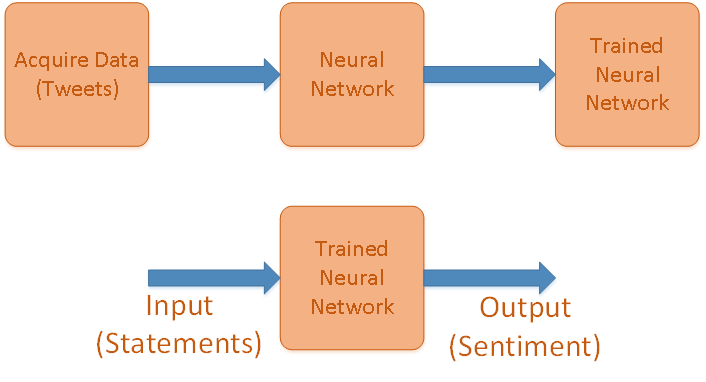
\includegraphics[width=4in]{Process.png}
        \end{center}
        \caption{The process of building a neural network.}
        \label{fig:NNProcess}
    \end{figure}

    Sentiment analysis is a special use case of neural networks. Sentiment (the view or attitude) of a piece of text is a hard problem to express in traditional programming and data science. There is no absolute way to express humor, happiness, or any other emotion. However, humans can understand and comprehend this. This is a problem suitable for machine learning.

    \subsection{Collecting Data}
    Data collection is a major part of machine learning. One method to get data is by pulling data from a public sources like Twitter. Twitter is a good source since the users tag their posts using hashtags. These hashtags can act like answer keys. For example, if a tweet uses the hashtag happy, it means the tweet represents happy sentiment.

    \subsection{Training}
    Training the neural network for sentiment analysis also has a major difficulty to overcome. Neural networks require large amounts of computation power to train. GPUs (Graphics Processing Units) which are used for training neural networks are very expensive. This makes training large neural networks very expensive. Training is also very time consuming since it has such a brute force approach and diminishing returns the longer you train. Refer to fig. ~\ref{fig:NNProcess} for a visual diagram of this process.

    \section{Conclusion}
    As part of this research, I was able to write scripts to collect a thousand tweets worth of data from Twitter for each of the sentiment hashtags that I was interested in.  I was also able to use Google's tool called TensorFlow to build and train my neural network consisting of 3 hidden layers each with 500 neurons.  I then created a front end where a user can input a sentence representing some kind of sentiment, and the script would use the trained neural network to identify the hidden emotion in the input sentence with fair accuracy.  In conclusion it is possible to use machine learning to identify emotions hidden in sentimental expressions. 

    \printbibliography
\end{document}
